\documentclass[english,a4paper,]{report}
\usepackage{lmodern}
\usepackage{amssymb,amsmath}
\usepackage{ifxetex,ifluatex}
\usepackage{fixltx2e} % provides \textsubscript
\ifnum 0\ifxetex 1\fi\ifluatex 1\fi=0 % if pdftex
  \usepackage[T1]{fontenc}
  \usepackage[utf8]{inputenc}
\else % if luatex or xelatex
  \ifxetex
    \usepackage{mathspec}
  \else
    \usepackage{fontspec}
  \fi
  \defaultfontfeatures{Ligatures=TeX,Scale=MatchLowercase}
\fi
% use upquote if available, for straight quotes in verbatim environments
\IfFileExists{upquote.sty}{\usepackage{upquote}}{}
% use microtype if available
\IfFileExists{microtype.sty}{%
\usepackage[]{microtype}
\UseMicrotypeSet[protrusion]{basicmath} % disable protrusion for tt fonts
}{}
\PassOptionsToPackage{hyphens}{url} % url is loaded by hyperref
\usepackage[unicode=true]{hyperref}
\hypersetup{
            pdftitle={Programming - Part I},
            pdfauthor={Ricard Solé Casas},
            pdfborder={0 0 0},
            breaklinks=true}
\urlstyle{same}  % don't use monospace font for urls
\usepackage[margin=1in]{geometry}
\ifnum 0\ifxetex 1\fi\ifluatex 1\fi=0 % if pdftex
  \usepackage[shorthands=off,main=english]{babel}
\else
  \usepackage{polyglossia}
  \setmainlanguage[]{english}
\fi
\usepackage{longtable,booktabs}
% Fix footnotes in tables (requires footnote package)
\IfFileExists{footnote.sty}{\usepackage{footnote}\makesavenoteenv{long table}}{}
\usepackage{graphicx,grffile}
\makeatletter
\def\maxwidth{\ifdim\Gin@nat@width>\linewidth\linewidth\else\Gin@nat@width\fi}
\def\maxheight{\ifdim\Gin@nat@height>\textheight\textheight\else\Gin@nat@height\fi}
\makeatother
% Scale images if necessary, so that they will not overflow the page
% margins by default, and it is still possible to overwrite the defaults
% using explicit options in \includegraphics[width, height, ...]{}
\setkeys{Gin}{width=\maxwidth,height=\maxheight,keepaspectratio}
% Make links footnotes instead of hotlinks:
\renewcommand{\href}[2]{#2\footnote{\url{#1}}}
\IfFileExists{parskip.sty}{%
\usepackage{parskip}
}{% else
\setlength{\parindent}{0pt}
\setlength{\parskip}{6pt plus 2pt minus 1pt}
}
\setlength{\emergencystretch}{3em}  % prevent overfull lines
\providecommand{\tightlist}{%
  \setlength{\itemsep}{0pt}\setlength{\parskip}{0pt}}
\setcounter{secnumdepth}{5}

% set default figure placement to htbp
\makeatletter
\def\fps@figure{htbp}
\makeatother

\usepackage{minted}
\usemintedstyle{autumn}

\usepackage{fontspec}
\setmonofont{Hasklig}
\defaultfontfeatures{Mapping=tex-text,Scale=MatchLowercase,Ligatures=TeX}

\title{Programming - Part I}
\author{Ricard Solé Casas}
\providecommand{\institute}[1]{}
\institute{Google UK \and Ada National College for Digital Skills}
\date{\today}

\begin{document}
\maketitle

\vspace*{\fill}

\section*{Foreword}

The source code for this report and app can be found on
\href{https://github.com/rcsole/coursework-java}{Github}. The live
version of the app itself is online at http://quiz.rsole.me.

Some of the decisions taken in building this app do not follow the
original suggested guidelines. The UI is a web frontend, but all the
business logic is handled by the server-side via Java.

\section*{Declaration}

I confirm that the submitted coursework is my own work and that all
material attributed to others (whether published or unpublished) has
been clearly identified and fully acknowledged and referred to original
sources. I agree that the College has the right to submit my work to the
plagiarism detection service. TurnitinUK for originality checks.

\section*{Acknowledgements}

I'd like to thank my partner Shannon for her continued support and
challenges that help me grow, both professionally and personally. I
would also like to thank all of you who also helped me get here.

\vspace*{\fill}

{
\setcounter{tocdepth}{2}
\tableofcontents
}
\chapter{Overview}\label{overview}

Project is setup using the Java \href{https://playframework.com}{Play}
framework to aid with following the
\href{https://www.wikiwand.com/en/Model\%E2\%80\%93view\%E2\%80\%93controller}{MVC}
pattern.

\section{Models}\label{models}

From Wikipedia:

\begin{quote}
\emph{The model is the central component of the pattern. It expresses
the application's behavior in terms of the problem domain, independent
of the user interface. It directly manages the data, logic and rules of
the application.}
\end{quote}

All the models used by this application are stored in
\href{https://www.postgresql.org/}{PostgreSQL}. The bindings are done
through
\href{https://www.playframework.com/documentation/2.5.x/JavaEbean}{PlayEbean}.

\subsection{Option}\label{option}

\texttt{Option} is the smallest model. It has a
\href{https://www.wikiwand.com/en/One-to-many_(data_model)}{one-to-many}
relationship to \protect\hyperlink{question}{\texttt{Question}}, where
one \texttt{Question} can have \texttt{n\ Option}s, and each
\texttt{Option} belongs to \texttt{1\ Question}.

In essence it's an alias to a \texttt{String} type, the only difference
is that \texttt{Option} has a \texttt{Long\ id} and a
\texttt{Question\ question}.

See \href{https://git.io/vHdem}{models/Option.java} for implementation.

\hypertarget{question}{\subsection{Question}\label{question}}

\texttt{Question} is, arguably, the meat of the application. It holds
\emph{many} \texttt{Option}s as a
\texttt{List\textless{}Option\textgreater{}}, along with other
parameters like difficulty, type, and category or the \texttt{Quiz} it
belongs to. Like \texttt{Option}, \texttt{Question} holds a
\href{https://www.wikiwand.com/en/One-to-many_(data_model)}{one-to-many}
relationship to \protect\hyperlink{quiz}{\texttt{Quiz}}. Except in this
case \texttt{n\ Question}s belong to \texttt{1\ Quiz}.

See \href{https://git.io/vHde6}{models/Question.java} for
implementation.

\hypertarget{quiz}{\subsection{Quiz}\label{quiz}}

This is the model that is actually used by other parts of the
application. The rest are intermediary models to store data in a way
that makes it easier to manipulate. \texttt{Quiz} owns two different
models, \texttt{QuizResult} and \texttt{Question}. Any \texttt{Quiz} may
have any number of \texttt{QuizResult}s and \texttt{Question}s.

It also has a \texttt{String\ difficulty} value which ranges from
\emph{easy} to \emph{hard}, or \emph{mixed}. Also provides a method int
\texttt{computeScore(DynamicForm\ answers)} to compute the score from a
form submission.

See \href{https://git.io/vHdvZ}{models/Quiz.java} for implementation.

\subsection{QuizResult}\label{quizresult}

\texttt{QuizResult} is how the application stores the return value of
\texttt{int\ computeScore(DynamicForm\ answers)} in \texttt{Quiz}. This
is to allow sharing and retaking the \texttt{Quiz}, hence the belonging
relationship.

See \href{https://git.io/vHdvn}{models/QuizResult.java} for
implementation.

\section{Services}\label{services}

\subsection{QuizService}\label{quizservice}

\section{Controllers}\label{controllers}

\subsection{QuizResultsController}\label{quizresultscontroller}

\subsection{QuizzesController}\label{quizzescontroller}

\chapter{Test plan}\label{test-plan}

\begin{longtable}[]{@{}llccc@{}}
\toprule
\begin{minipage}[b]{0.16\columnwidth}\raggedright\strut
\emph{Test}\strut
\end{minipage} & \begin{minipage}[b]{0.15\columnwidth}\raggedright\strut
\emph{Method}\strut
\end{minipage} & \begin{minipage}[b]{0.19\columnwidth}\centering\strut
\emph{Expected}\strut
\end{minipage} & \begin{minipage}[b]{0.17\columnwidth}\centering\strut
\emph{Actual}\strut
\end{minipage} & \begin{minipage}[b]{0.18\columnwidth}\centering\strut
\emph{Evidence}\strut
\end{minipage}\tabularnewline
\midrule
\endhead
\begin{minipage}[t]{0.16\columnwidth}\raggedright\strut
Selecting 10 creates a quiz with 10 questions\strut
\end{minipage} & \begin{minipage}[t]{0.15\columnwidth}\raggedright\strut
Click 10\strut
\end{minipage} & \begin{minipage}[t]{0.19\columnwidth}\centering\strut
There will be 10 questions\strut
\end{minipage} & \begin{minipage}[t]{0.17\columnwidth}\centering\strut
As expected\strut
\end{minipage} & \begin{minipage}[t]{0.18\columnwidth}\centering\strut
See figure \ref{fig:1}\strut
\end{minipage}\tabularnewline
\begin{minipage}[t]{0.16\columnwidth}\raggedright\strut
Selecting 20 creates a quiz with 20 questions\strut
\end{minipage} & \begin{minipage}[t]{0.15\columnwidth}\raggedright\strut
Click 20\strut
\end{minipage} & \begin{minipage}[t]{0.19\columnwidth}\centering\strut
There will be 20 questions\strut
\end{minipage} & \begin{minipage}[t]{0.17\columnwidth}\centering\strut
As expected\strut
\end{minipage} & \begin{minipage}[t]{0.18\columnwidth}\centering\strut
See figure \ref{fig:2}\strut
\end{minipage}\tabularnewline
\begin{minipage}[t]{0.16\columnwidth}\raggedright\strut
Selecting 30 creates a quiz with 30 questions\strut
\end{minipage} & \begin{minipage}[t]{0.15\columnwidth}\raggedright\strut
Click 30\strut
\end{minipage} & \begin{minipage}[t]{0.19\columnwidth}\centering\strut
There will be 30 questions\strut
\end{minipage} & \begin{minipage}[t]{0.17\columnwidth}\centering\strut
As expected\strut
\end{minipage} & \begin{minipage}[t]{0.18\columnwidth}\centering\strut
See figure \ref{fig:3}\strut
\end{minipage}\tabularnewline
\begin{minipage}[t]{0.16\columnwidth}\raggedright\strut
Cross on top left takes user back to quiz creation\strut
\end{minipage} & \begin{minipage}[t]{0.15\columnwidth}\raggedright\strut
Click \texttt{x}\strut
\end{minipage} & \begin{minipage}[t]{0.19\columnwidth}\centering\strut
Quiz will go back to form\strut
\end{minipage} & \begin{minipage}[t]{0.17\columnwidth}\centering\strut
As expected\strut
\end{minipage} & \begin{minipage}[t]{0.18\columnwidth}\centering\strut
See gif\footnotemark{}\strut
\end{minipage}
\footnotetext{http://www.giphy.com/gifs/3ohzdEZt9v5mq8oAsE}\tabularnewline
\begin{minipage}[t]{0.16\columnwidth}\raggedright\strut
Selecting an option brings the next question up\strut
\end{minipage} & \begin{minipage}[t]{0.15\columnwidth}\raggedright\strut
Select an option\strut
\end{minipage} & \begin{minipage}[t]{0.19\columnwidth}\centering\strut
Next question will come up\strut
\end{minipage} & \begin{minipage}[t]{0.17\columnwidth}\centering\strut
As expected\strut
\end{minipage} & \begin{minipage}[t]{0.18\columnwidth}\centering\strut
See gif\footnotemark{}\strut
\end{minipage}
\footnotetext{http://www.giphy.com/gifs/3og0IMCTcnr7RFvaaQ}\tabularnewline
\begin{minipage}[t]{0.16\columnwidth}\raggedright\strut
Skipping will send the question to the end\strut
\end{minipage} & \begin{minipage}[t]{0.15\columnwidth}\raggedright\strut
Skip a question\strut
\end{minipage} & \begin{minipage}[t]{0.19\columnwidth}\centering\strut
The question will be skipped and asked again at the end of the
quiz\strut
\end{minipage} & \begin{minipage}[t]{0.17\columnwidth}\centering\strut
As expected\strut
\end{minipage} & \begin{minipage}[t]{0.18\columnwidth}\centering\strut
See gif\footnotemark{}\strut
\end{minipage}
\footnotetext{http://www.giphy.com/gifs/l1BgSVSrual0DUzDi}\tabularnewline
\begin{minipage}[t]{0.16\columnwidth}\raggedright\strut
When the timer runs out the quiz gets submitted\strut
\end{minipage} & \begin{minipage}[t]{0.15\columnwidth}\raggedright\strut
Wait for timer to run out\strut
\end{minipage} & \begin{minipage}[t]{0.19\columnwidth}\centering\strut
The quiz gets submitted\strut
\end{minipage} & \begin{minipage}[t]{0.17\columnwidth}\centering\strut
As expected\strut
\end{minipage} & \begin{minipage}[t]{0.18\columnwidth}\centering\strut
See gif\footnotemark{}\strut
\end{minipage}
\footnotetext{http://www.giphy.com/gifs/l0Iy8yTqqq5BCf1yU}\tabularnewline
\begin{minipage}[t]{0.16\columnwidth}\raggedright\strut
Score is displayed as a percentage\strut
\end{minipage} & \begin{minipage}[t]{0.15\columnwidth}\raggedright\strut
Finish the quiz\strut
\end{minipage} & \begin{minipage}[t]{0.19\columnwidth}\centering\strut
The score is displayed upon finishing the quiz\strut
\end{minipage} & \begin{minipage}[t]{0.17\columnwidth}\centering\strut
As expected\strut
\end{minipage} & \begin{minipage}[t]{0.18\columnwidth}\centering\strut
See figure \ref{fig:4}\strut
\end{minipage}\tabularnewline
\bottomrule
\end{longtable}

\begin{figure}
\centering
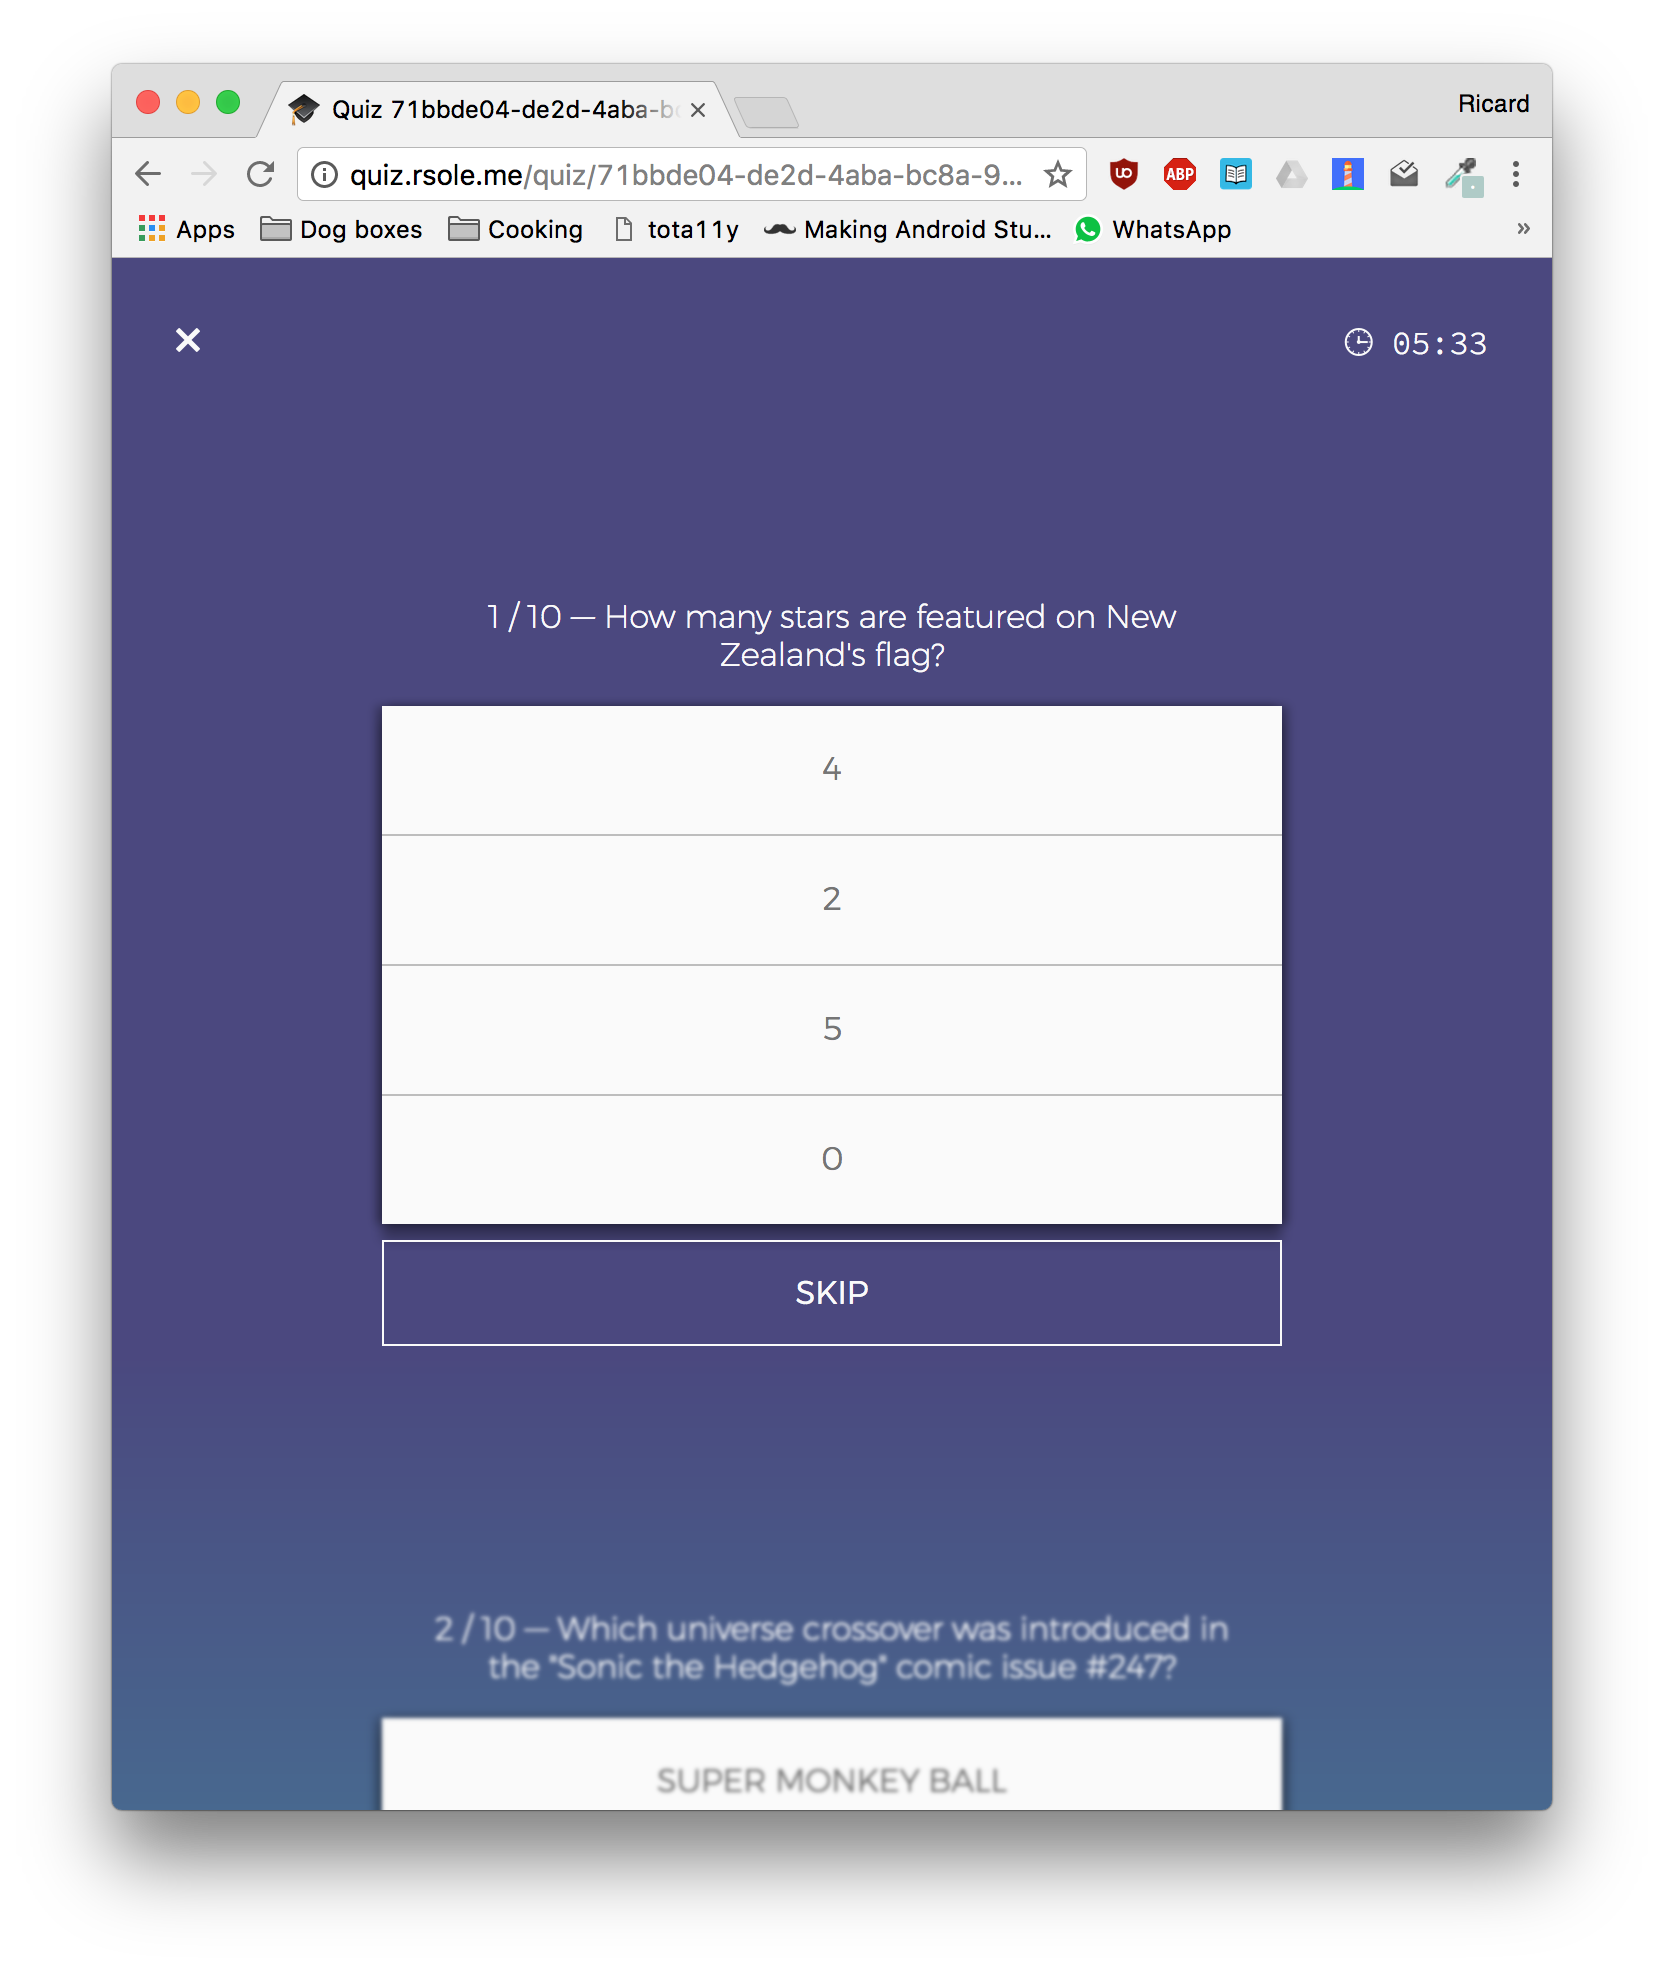
\includegraphics{report/images/00.png}
\caption{10 Questions\label{fig:1}}
\end{figure}

\begin{figure}
\centering
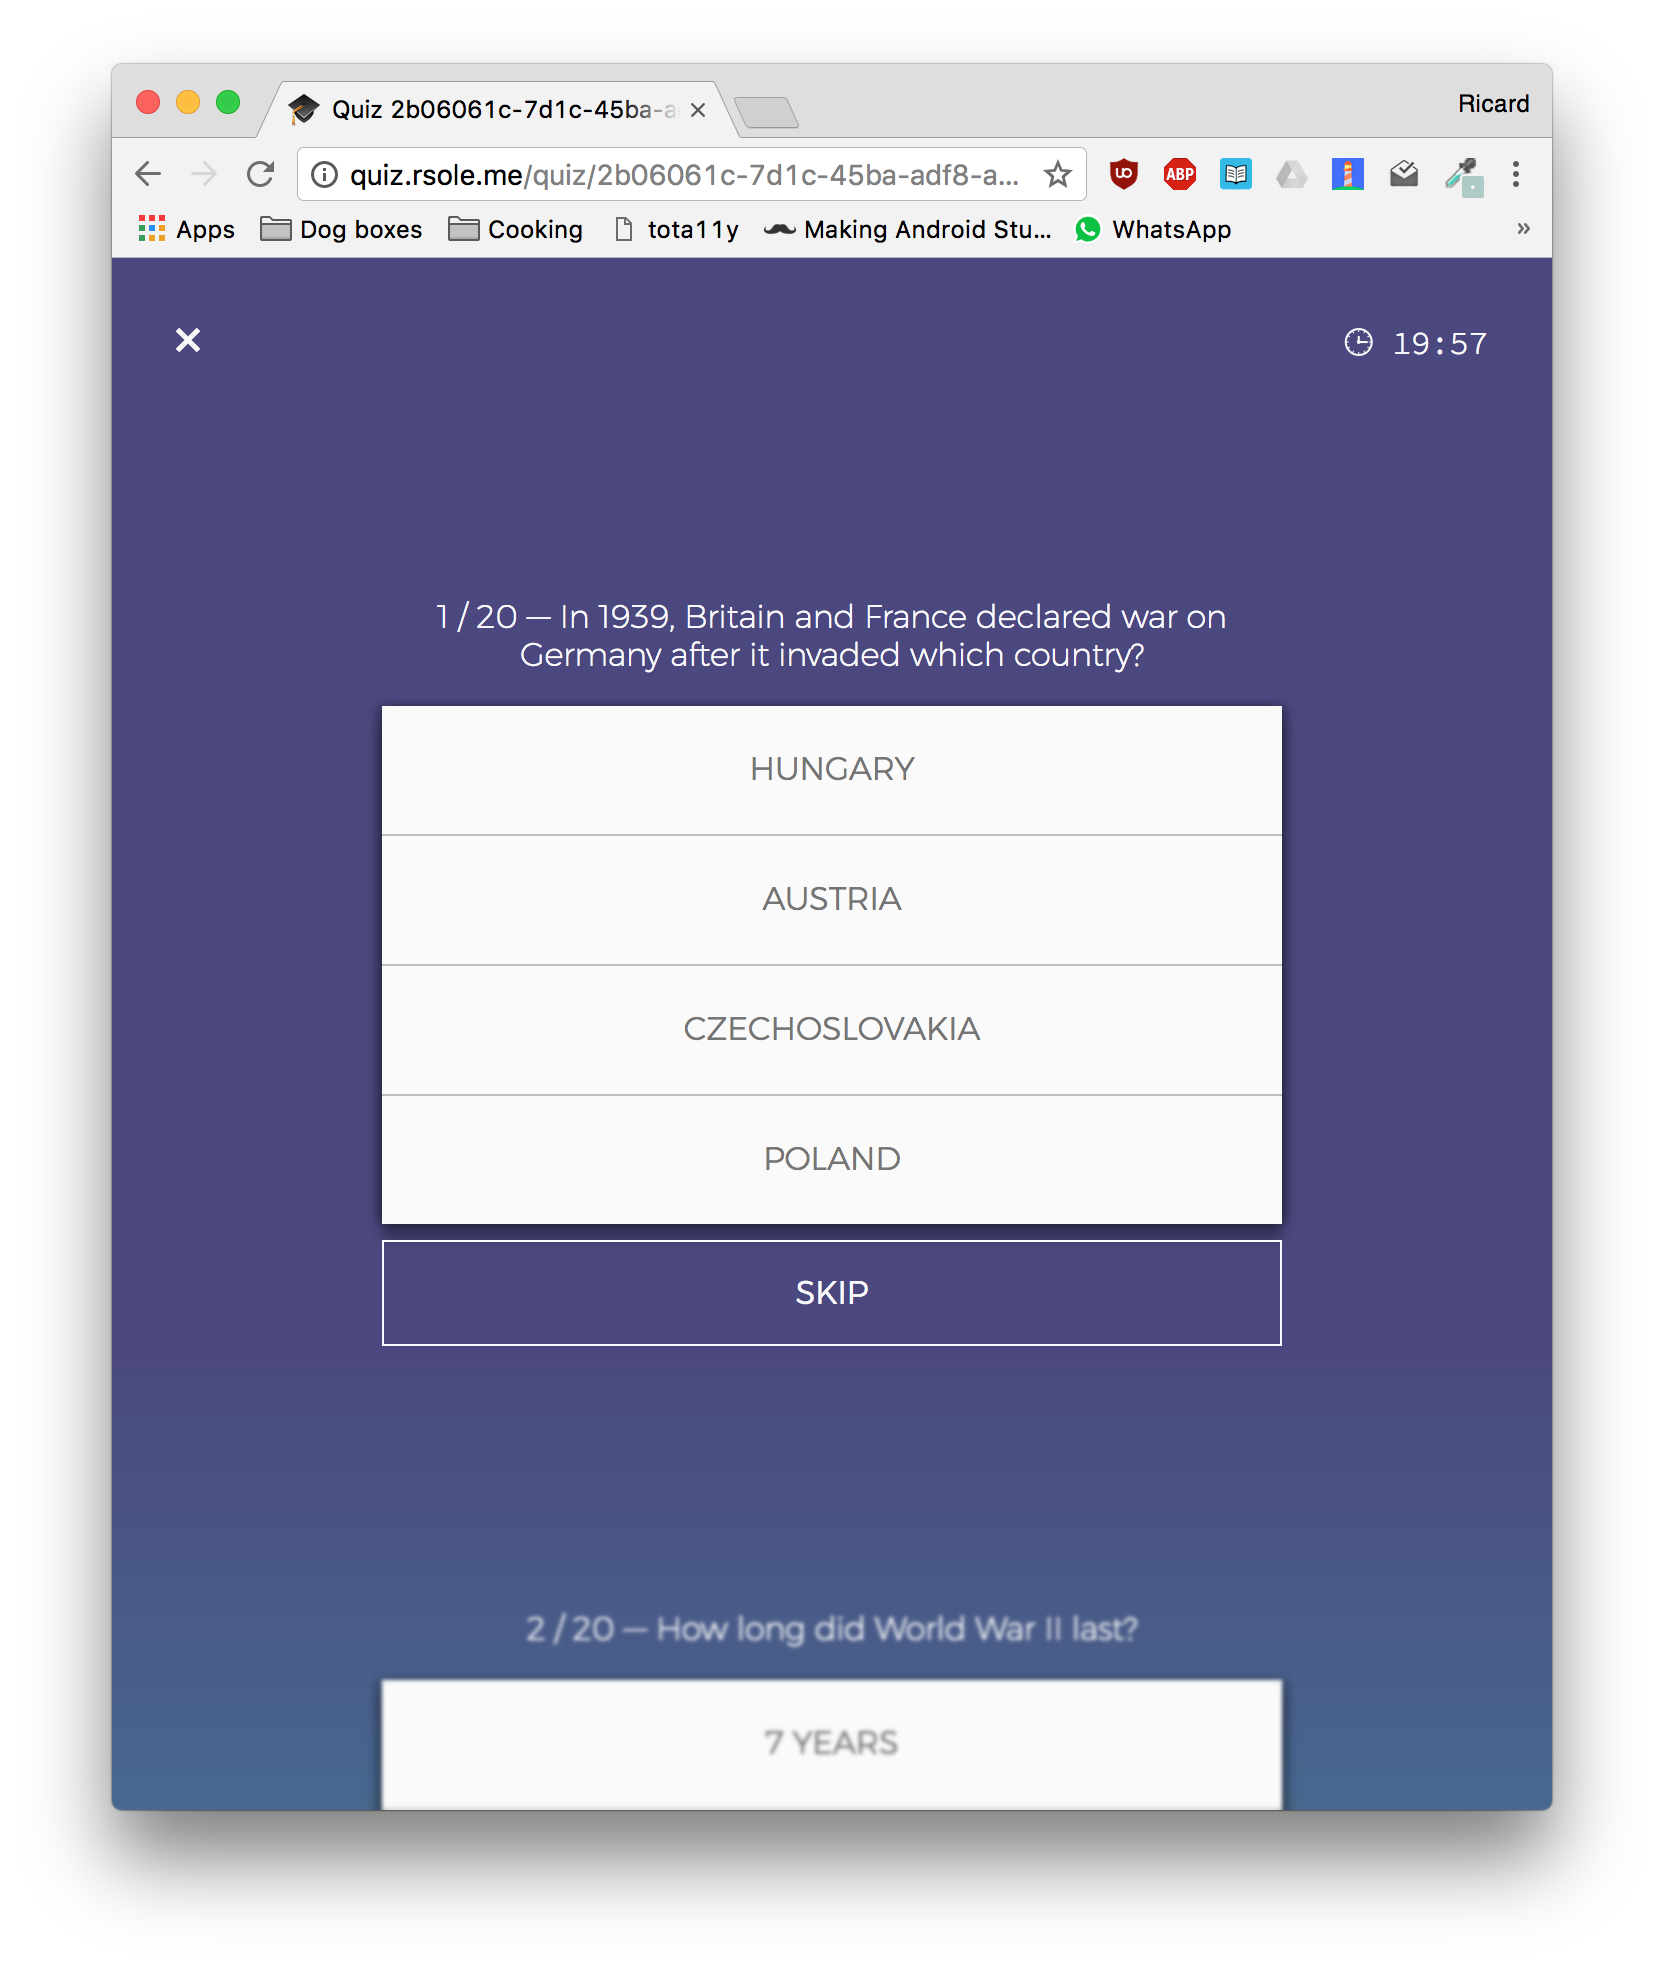
\includegraphics{report/images/01.png}
\caption{20 Questions\label{fig:2}}
\end{figure}

\begin{figure}
\centering
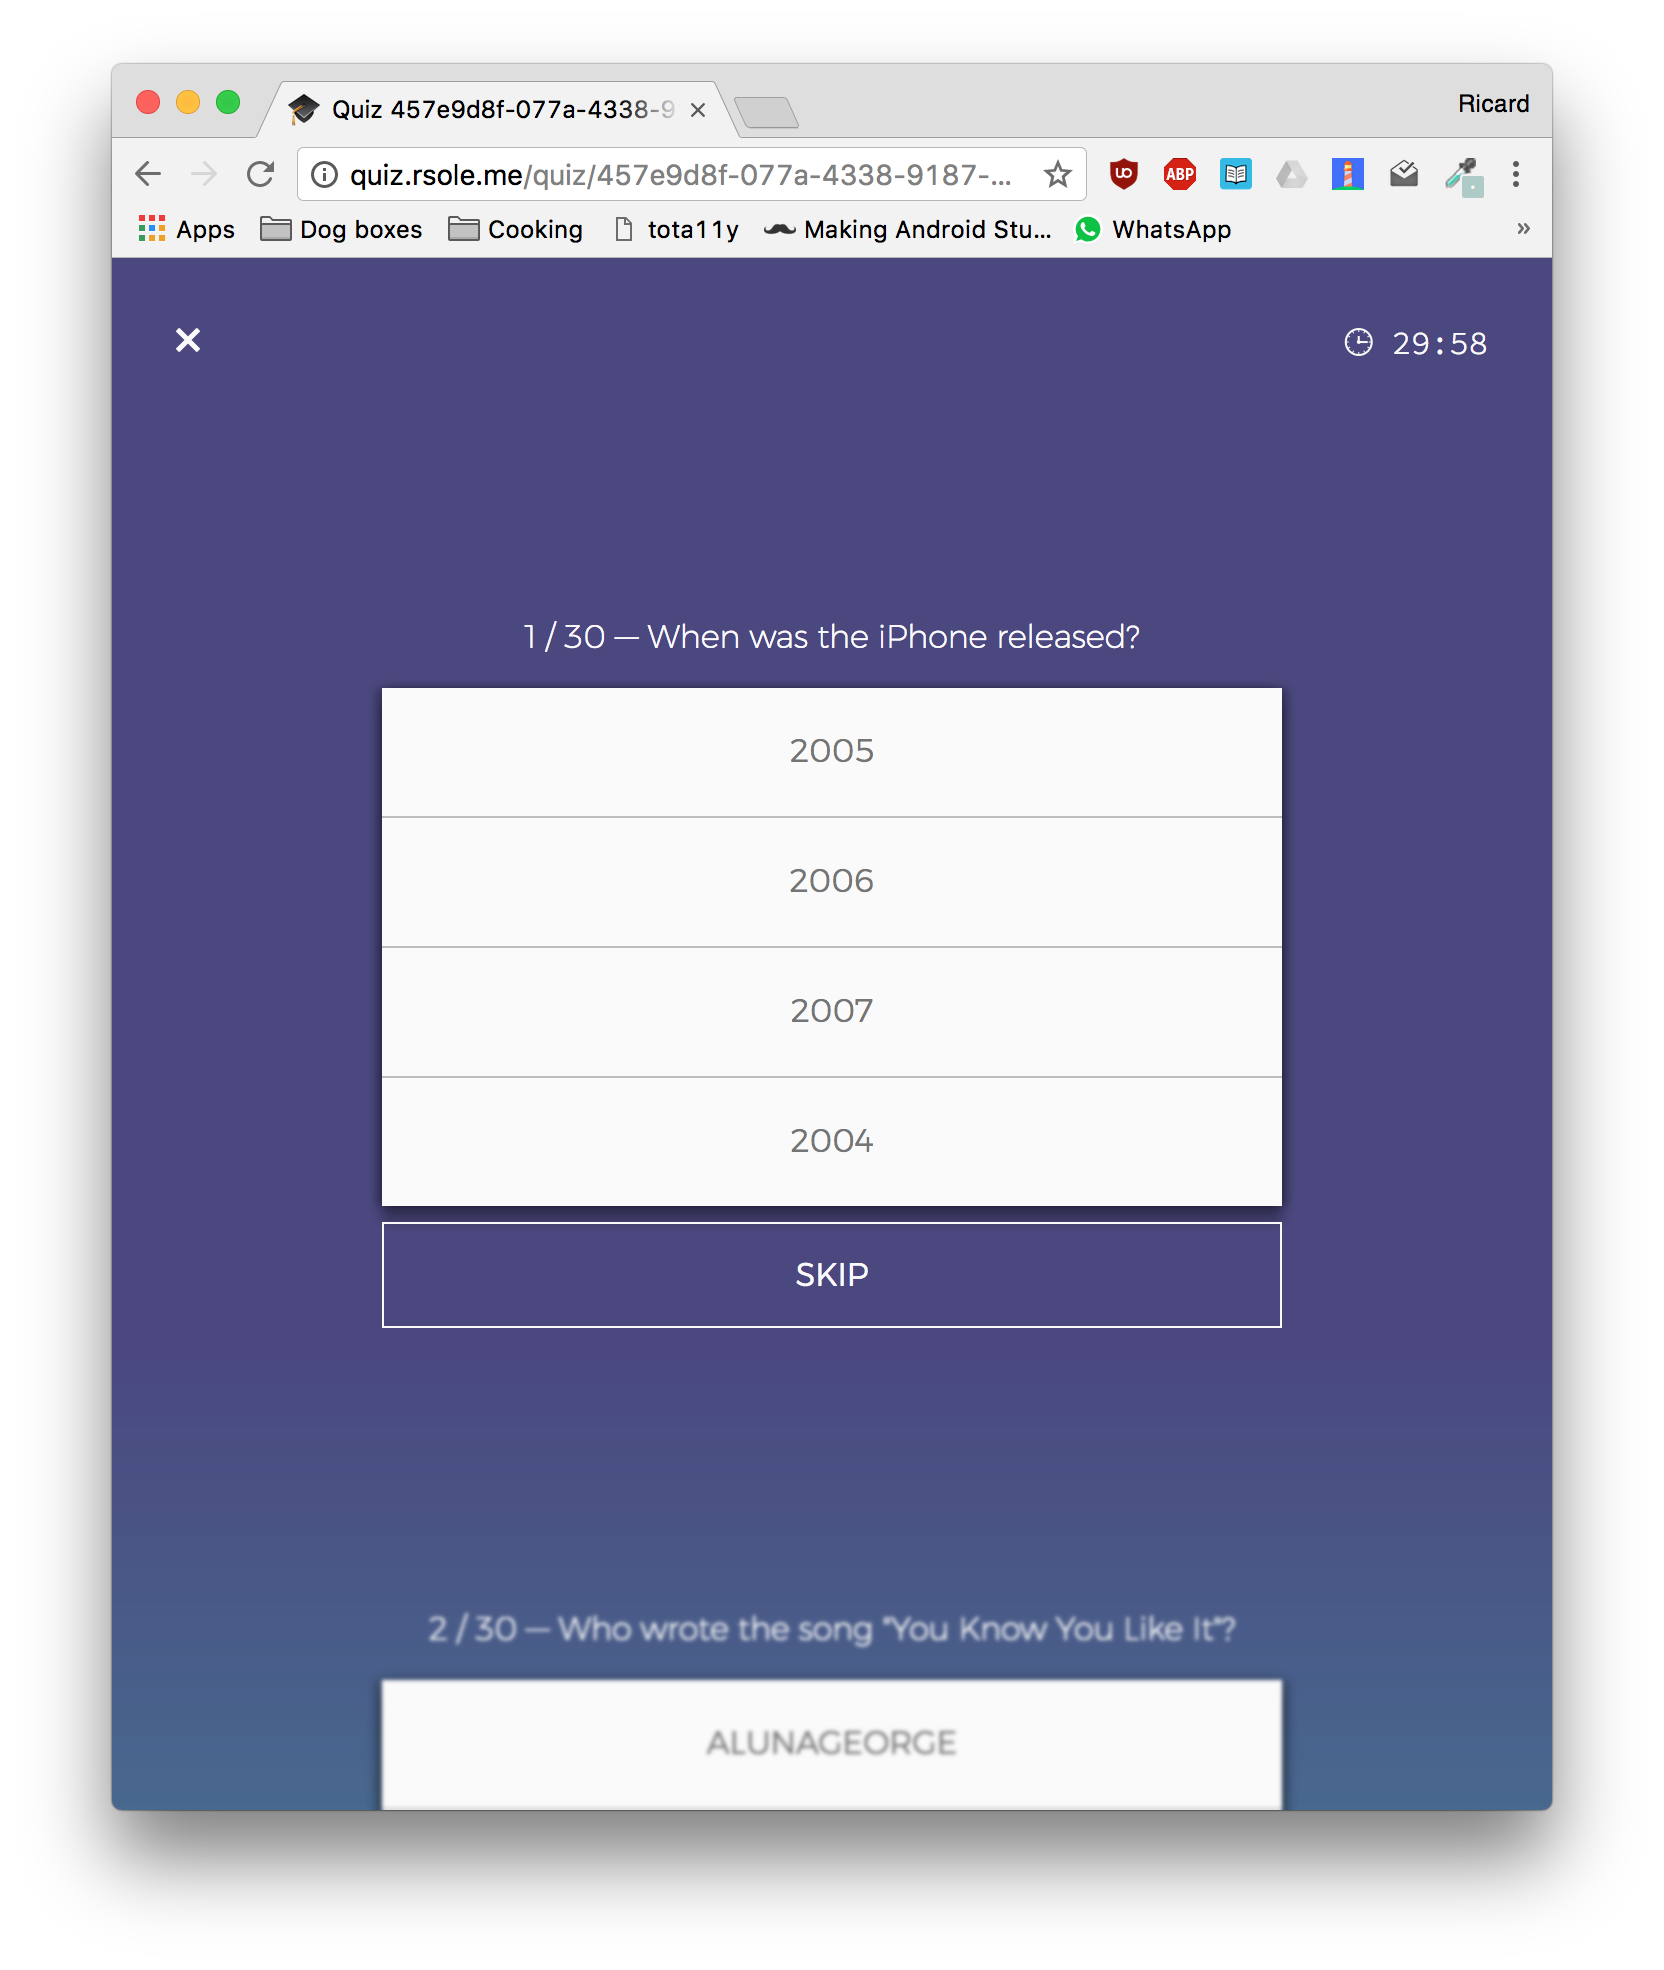
\includegraphics{report/images/02.png}
\caption{30 Questions\label{fig:3}}
\end{figure}

\begin{figure}
\centering
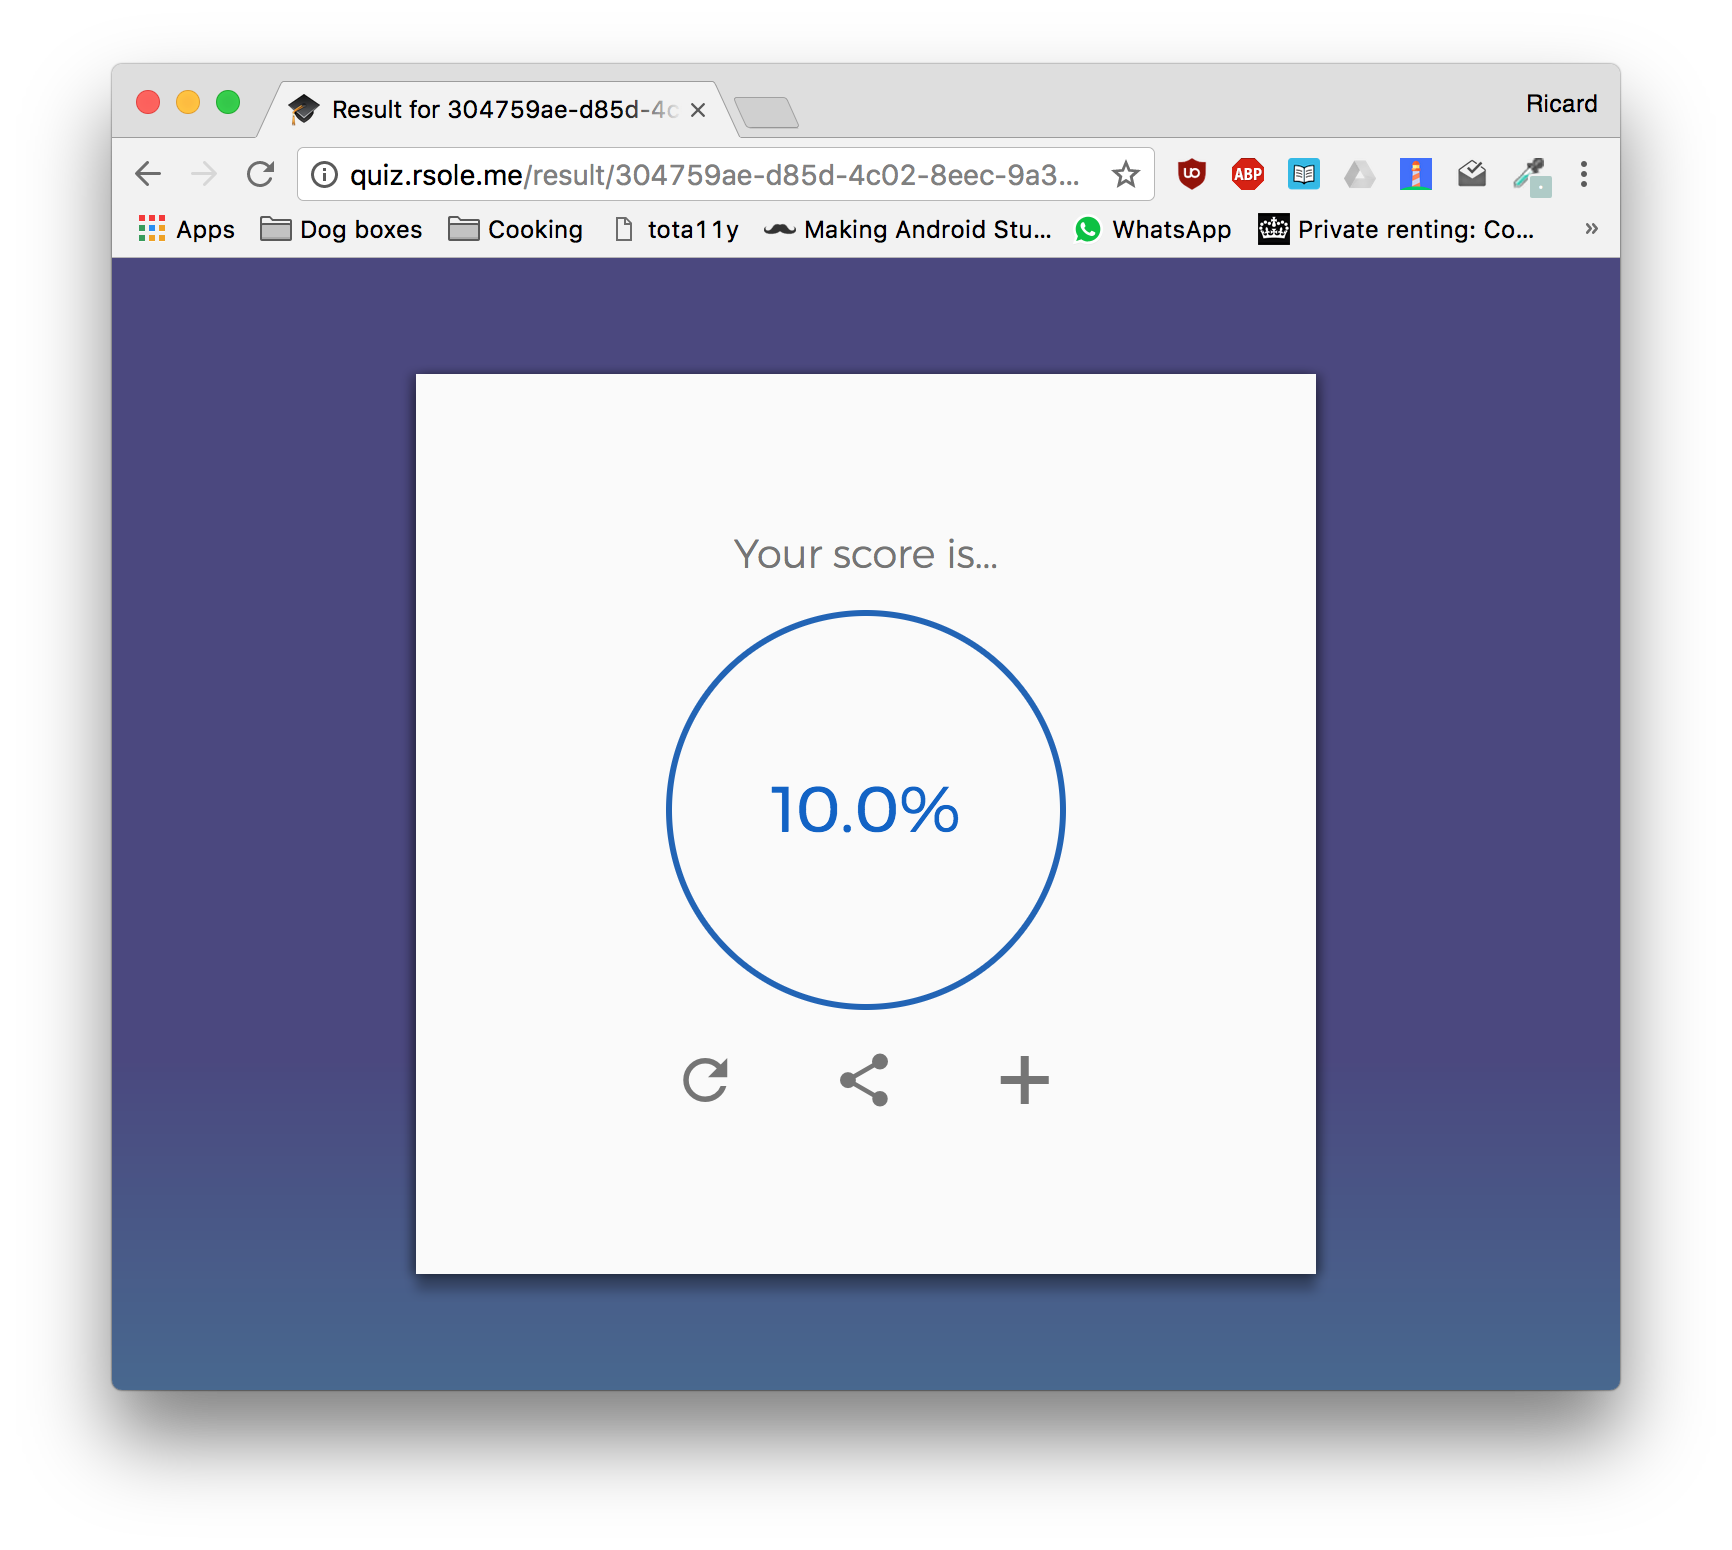
\includegraphics{report/images/03.png}
\caption{Quiz result\label{fig:4}}
\end{figure}

\chapter{Appendix A: Source Code}\label{appendix-a-source-code}

\section{QuizResultsController.java}\label{quizresultscontroller.java}

\inputminted{java}{app/controllers/QuizResultsController.java}

\section{QuizzesController.java}\label{quizzescontroller.java}

\inputminted{java}{app/controllers/QuizzesController.java}

\section{Option.java}\label{option.java}

\inputminted{java}{app/models/Option.java}

\section{Question.java}\label{question.java}

\inputminted{java}{app/models/Question.java}

\section{Quiz.java}\label{quiz.java}

\inputminted{java}{app/models/Quiz.java}

\section{QuizResult.java}\label{quizresult.java}

\inputminted{java}{app/models/QuizResult.java}

\section{QuizService.java}\label{quizservice.java}

\inputminted{java}{app/services/QuizService.java}

\end{document}
